% Replacement for figures/motivation.tex in the v14 Overleaf project.
% Requires tikz, xcolor, graphicx and arrows.meta (already loaded by main.tex).
\begin{figure*}[t]
\centering
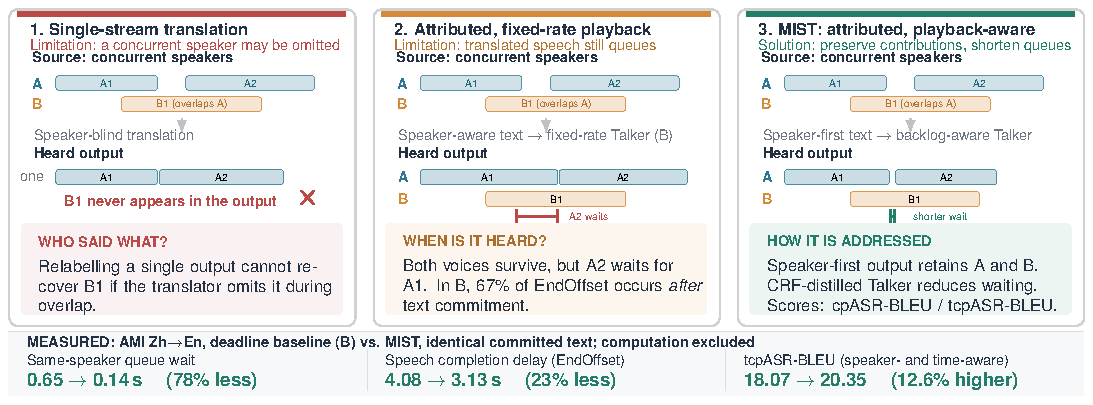
\includegraphics[height=5cm]{figures/MIST_Figure1_Motivation_Redesigned.pdf}
\caption{Motivation. (1)~Speaker-blind single-stream translation may omit overlapping contributions. (2)~Speaker attribution alone leaves playback queues: 67\% of the deadline baseline's EndOffset occurs after text commitment (queue plus final-block playback; Table~\ref{tab:decomp}). (3)~\sys{} combines speaker-first decoding with a backlog-aware Talker trained on the posterior of a playback-queue CRF; no CRF runs online. Bottom: measured improvements on AMI Zh$\rightarrow$En over the baseline with identical text, excluding computation. All utterance timelines are schematic.}
\label{fig:motivation}

\end{figure*}
